% helpful source: https://www.pctex.com/kb/64.html
% http://www.cpt.univ-mrs.fr/~masson/latex/Beamer-appearance-cheat-sheet.pdf

\documentclass[]{beamer}
% Class options include: notes, notesonly, handout, trans,
%                        hidesubsections, shadesubsections,
%                        inrow, blue, red, grey, brown

% Theme for beamer presentation.
%\usepackage{beamerthemesplit} 
\usepackage{beamerthemebars}
% Other themes include: beamerthemebars, beamerthemelined, 
%                       beamerthemetree, beamerthemetreebars  

\usetheme{Copenhagen}
%\usetheme{AnnArbor}
\usecolortheme{beaver}

\graphicspath{{images/}}  


% My other suggestion for color: violet!64!white 

\setbeamercolor{titlelike}{parent=structure,bg=violet!34!white,fg=black}

\setbeamercolor{title}{parent=structure,bg=violet!34!white,fg=black}

\setbeamercolor{section in toc}{parent=structure,fg=violet}

\setbeamercolor{section in head/foot}{parent=structure,bg=violet!34!white,fg=black}

\setbeamercolor{title in head/foot}{parent=structure,bg=white,fg=black}

\setbeamercolor{author in head/foot}{parent=structure,bg=violet!34!white,fg=black}

%\setbeamercolor{page number in head/foot}{parent=structure,bg=violet}

\setbeamercolor{subsection in head/foot}{parent=structure,bg=black!10!white,fg=black}

\setbeamercolor{item}{parent=structure,bg=violet!34!white,fg=black}


\newcommand{\backupbegin}{
   \newcounter{finalframe}
   \setcounter{finalframe}{\value{framenumber}}
}
\newcommand{\backupend}{
   \setcounter{framenumber}{\value{finalframe}}
}





\title{Deep Neural Network for Multi-Hop Question Answering}    
\author{Faeze Zakaryapour Sayyad \\ {\tiny Supervisor: Mahdi Bohlouli } }
\institute{The Institute for Advanced Studies in Basic Sciences}      
\date{September 22, 2021}  % Enter the date or \today 
\logo{

\includegraphics[width=3cm]{_LOGOIASBS_EN.png}
}


\begin{document}

\setbeamertemplate{footline}[frame number]

% Creates title page of slide show using above information
\begin{frame}
  \titlepage
\end{frame}
\note{Talk for 30 minutes} % Add notes to yourself that will be displayed when
                           % typeset with the notes or notesonly class options

\section[Outline]{}

% Creates table of contents slide incorporating
% all \section and \subsection commands
\begin{frame}
  \tableofcontents
\end{frame}


% -----------------------------------------INTRODUCTION------------------------------------
\section{Introduction}

\begin{frame}
\frametitle{Introduction}   % Insert frame title between curly braces


\begin{minipage}{4cm}

\includegraphics[height=3.5cm, width=3.5cm]{1.png} \\
\centering
\tiny{ { \color{gray} https://pinngle.me/blog/20-amazing-facts-to-know-about-chatbots/}}

\end{minipage}%
\begin{minipage}{7cm}
\textbf{Question Answering (QA)}  focuses on building QA systems by giving the ability to the computer to understand human’s questions and answer them based on some methods.

\end{minipage}
  
\end{frame}


\subsection{Open-domain vs. Closed-domain}
\begin{frame}
\frametitle{Open-domain vs. Closed-domain}

\begin{itemize}
\item Open-domain QA refers to systems that answer any domain-independent question.

\item Closed-domain QA systems only answer questions from a specific domain.

\end{itemize}
\end{frame}

\note[enumerate]       % Add notes to yourself that will be displayed when
{                      % typeset with the notes or notesonly class options
\item Example 1
\item Example 2
}


\subsection{Supporting Information}
\begin{frame}
\frametitle{Supporting Information}

\begin{itemize}
\item%<1->
Text-based: Supporting information is raw text, and hence the query is also text.


\item%<2-> 
Knowledge-based: Supporting information is from structured knowledge bases (KBs) but the queries can be either structured or natural language utterances.

\item%<3->
Mixed: Mixed QA tasks combine both text and KBs.

\end{itemize}

\end{frame}


\subsection{Single-hop vs. Multi-hop}

\begin{frame}
\frametitle{Single-hop vs. Multi-hop} 

\begin{itemize}

\item<1-> Single-hop QA: Only requires one fact to answer a question.
  \begin{itemize}
	 \item<2-> Example: What is the capital city of Iran?
  \end{itemize}

  
\item<3-> Multi-hop QA: Requires identifying multiple related facts and reasoning about them.
\begin{itemize}
	 \item<4-> Example: What is the capital city of the largest state in the Asia?  
  \end{itemize}
  
  \end{itemize}
  
  
\end{frame}


% ---------------------------- The focus of your work -----------------------------------------
\begin{frame}

\begin{minipage}{4cm}

\includegraphics[height=3.5cm, width=3.5cm]{2.jpg} \\
\centering 
\tiny{ {\color{gray} http://www.rte.ie/brainstorm/2021/0218/1197882-ireland-artificial-intelligence-strategy-ai/}}

\end{minipage}%
\begin{minipage}{7cm}
\begin{itemize}
\item Open-domain text-based question answering 
\item Questions can be both single- and multi-hop
\end{itemize}
\end{minipage}

\end{frame}


% ---------------------------------------------RELATED WORK----------------------------------------
\section{Related work}

\subsection{DrQA}
\begin{frame}
\frametitle{Reading Wikipedia to Answer Open-Domain Questions}


\centering
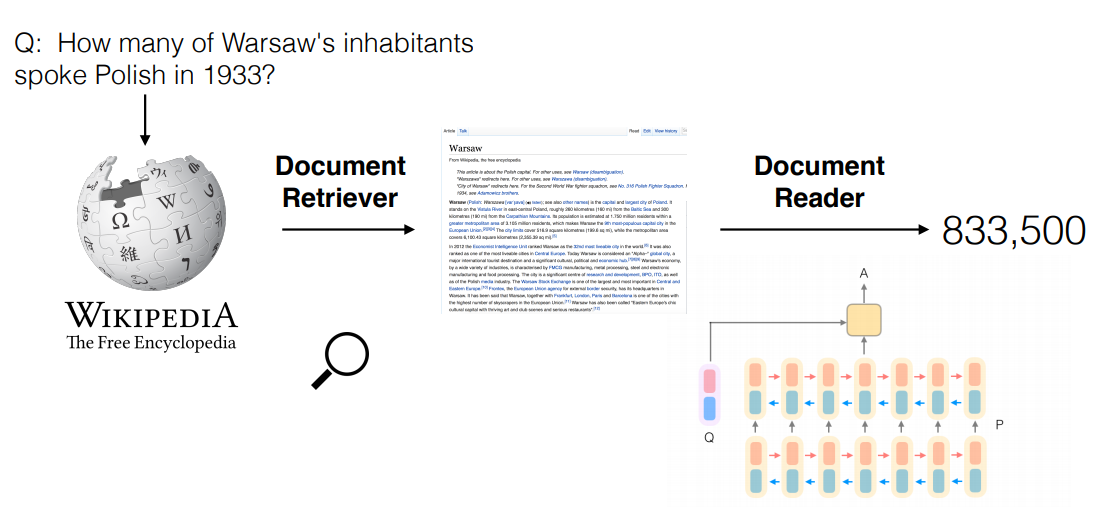
\includegraphics[scale=0.24]{2.png}

\centering
\tiny{{ \color{gray}Chen, D., Fisch, A., Weston, J., \& Bordes, A. (2017, July). Reading Wikipedia to Answer Open-Domain Questions. In Proceedings of the 55th Annual Meeting of the Association for Computational Linguistics (Volume 1: Long Papers) (pp. 1870-1879).}}

\end{frame}

\subsection{MUPPET}
\begin{frame}
\frametitle{Multi-Hop Paragraph Retrieval for Open-Domain Question Answering}

\centering
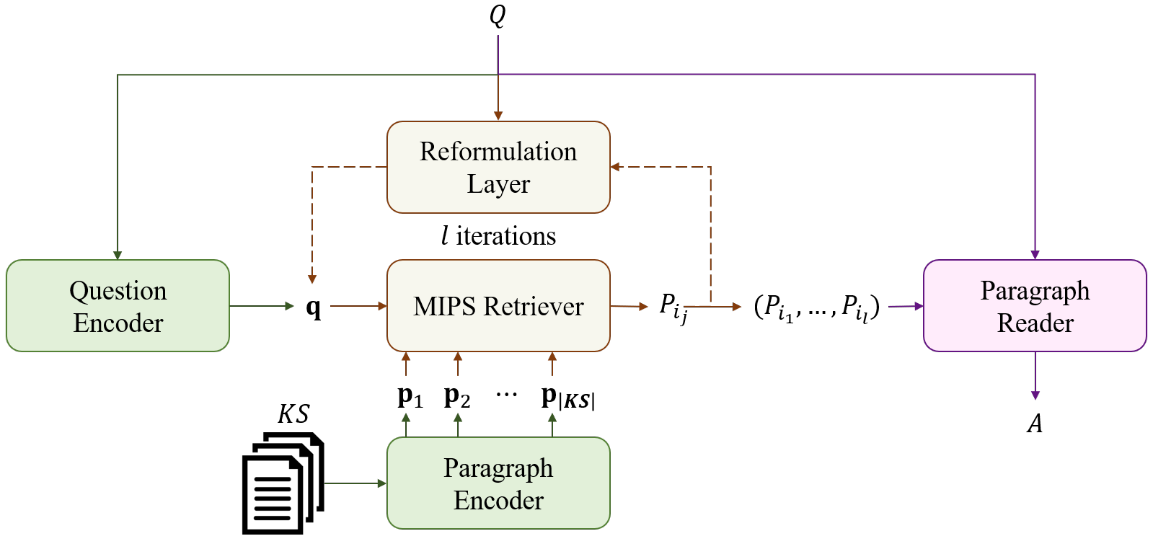
\includegraphics[scale=0.21]{3.png}


\centering
\tiny{ {\color{gray}Feldman, Y., \& El-Yaniv, R. (2019). Multi-hop paragraph retrieval for open-domain question answering. arXiv preprint arXiv:1906.06606.}}

\end{frame}


\subsection{Multi-Hop QA Systems' Failure}
\begin{frame}
\frametitle{Do Multi-Hop Question Answering Systems Know How to Answer the Single-Hop Sub-Questions?}

\centering
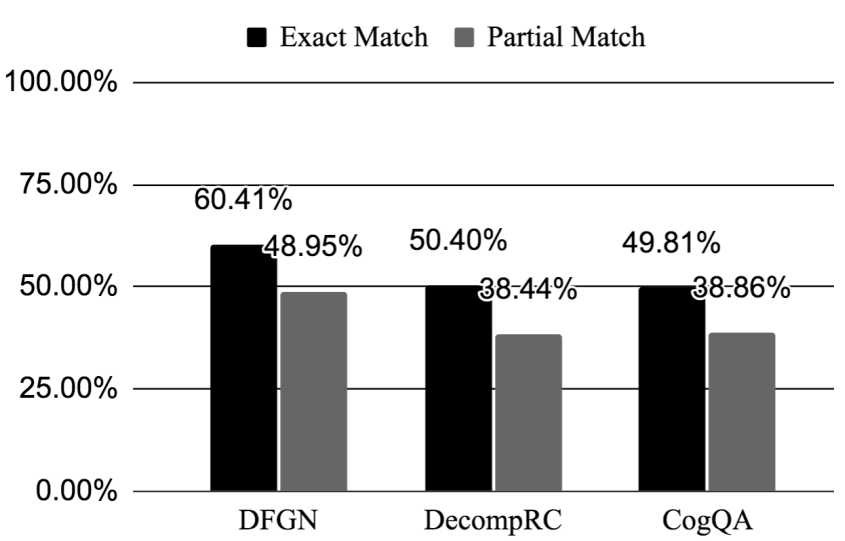
\includegraphics[scale=0.16]{4.png}

\centering
\tiny{Model failure rates under EM and PM.}
\bigskip

\tiny{ {\color{gray} Tang, Y., Ng, H. T., \& Tung, A. (2021, April). Do Multi-Hop Question Answering Systems Know How to Answer the Single-Hop Sub-Questions?. In Proceedings of the 16th Conference of the European Chapter of the Association for Computational Linguistics: Main Volume (pp. 3244-3249).}}

\end{frame}




% ----------------------------------------------YOUR WORK-------------------------------------
\section{Our Work}


\subsection{Datasets}
\begin{frame}
\frametitle{Datasets}

\begin{itemize}
\item SQuAD: Single-hop dataset
% Stanford University
\item HotpotQA: Multi-hop dataset
% Carnegie Mellon University, Stanford University, and Université de Montréal.
\item SiMhop: Mix dataset
\end{itemize}

\end{frame}


\subsection{Proposed Architecture}

\begin{frame}
Here you can add the detail of your proposed architecture and methods.
\end{frame}

 %---------------------------------------------------------------RESULTS----------------------------------------
\section{Results}

\begin{frame}
Here you can add the table of your results.
\end{frame}

% ---------------------------------------------------------------CONCLUSION-----------------------------------
 
\section{Conclusion}
\begin{frame}
\frametitle{Conclusion}

\begin{itemize}
\item Conclude your presentation
\item Talk about future works
\end{itemize}
\end{frame}

\begin{frame}

\bigskip
\bigskip
\bigskip
\bigskip

\centering
Thank you for your attention

\bigskip
\bigskip
\bigskip
\bigskip
\bigskip

\centering
\tiny{Email: Faezehzps@gmail.com} 
\end{frame}

% ---------------------------------------------------------------Appendix----------------------------------------

\appendix

\backupbegin
\section{More details}

\subsection{Detail of different parts of your presentation}
\begin{frame}
\frametitle{Extra pages}
You can add extra pages here, without numerating them in total number of pages.
\end{frame}

\backupend

\end{document}
